\section{Test-Überschrift}
\section{Auswertung}
\subsection{Rekonstruktionsalgoritmen}
\begin{figure}[h!]
	\centering
	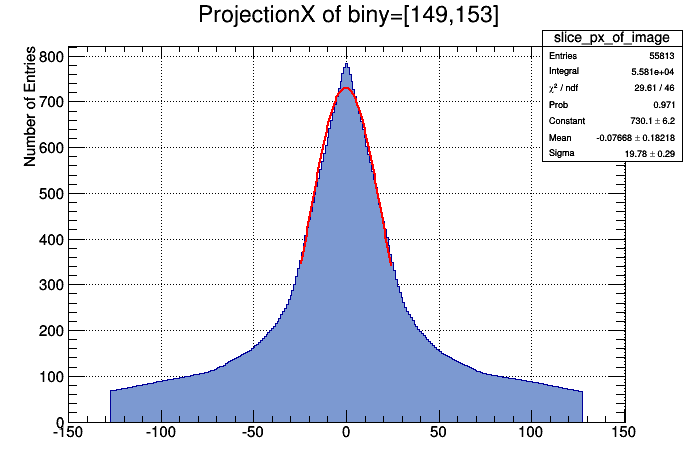
\includegraphics[width=0.9\textwidth]{Ohne-Filter.png}
	\caption{}
	\label{}
\end{figure}
\begin{figure}[h!]
	\centering
	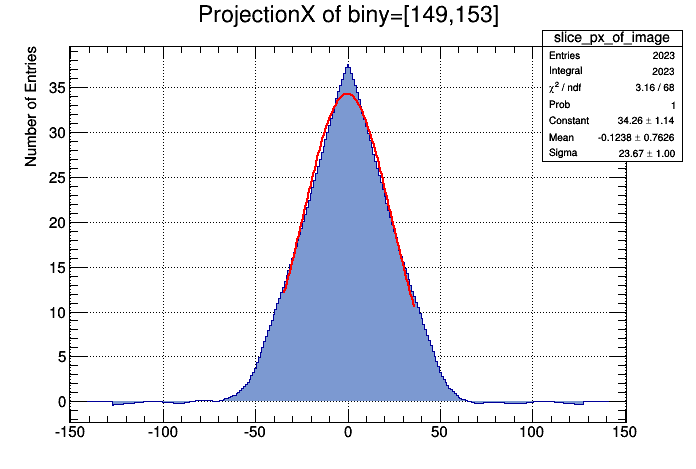
\includegraphics[width=0.9\textwidth]{Hann-Filter.png}
	\caption{}
	\label{}
\end{figure}
\begin{figure}[h!]
	\centering
	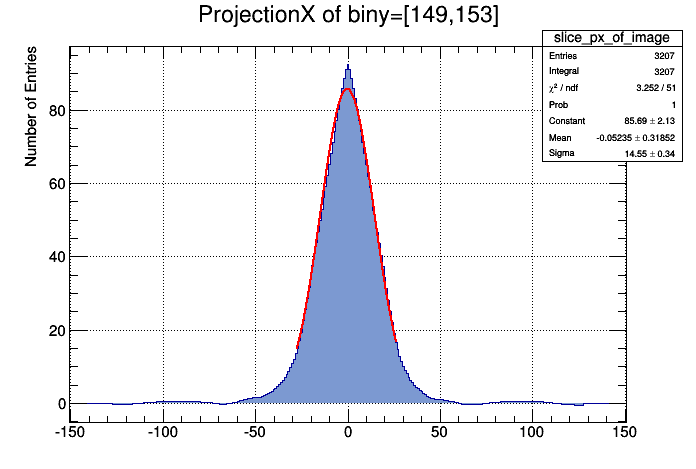
\includegraphics[width=0.9\textwidth]{Shepp-Logan-Filter.png}
	\caption{}
	\label{}
\end{figure}
\begin{figure}[h!]
	\centering
	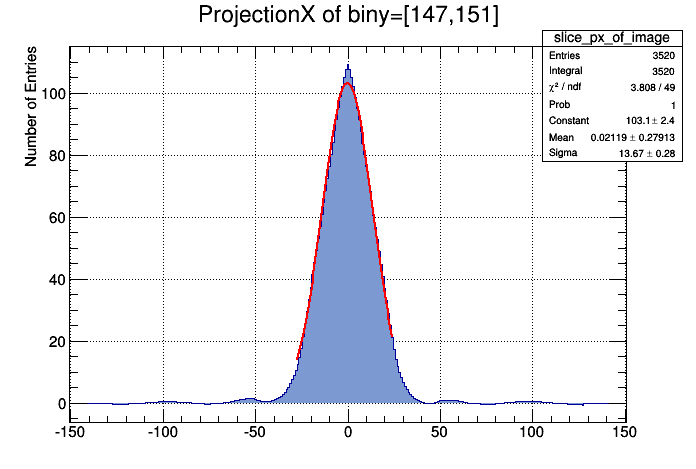
\includegraphics[width=0.9\textwidth]{Ramp-Filter.png}
	\caption{}
	\label{}
\end{figure}


\begin{tabular}{|c|c|c|c|}
	\hline 
	Algorithmus & Sigma & FWHM (keV) & Unsicherheiten FWHM (keV) \\ 
	\hline 
	pixel driven backprojection & 19,8 & 46,5 & 0,3 \\ 
	\hline 
	filtered backprojection Hann & 23.0 & 54 & 1  \\ 
	\hline 
	filtered backprojection Shepp-Logan & 14,4 & 33,8 & 0,3 \\ 
	\hline 
	filtered backprojektion Ramp & 13,7 & 39,2 & 0,3 \\ 
	\hline 
\end{tabular} 

\subsection{Positionsbestimmung}


\subsection{Auflösungsvermögen}